\definecolor{cfwone}{HTML}{eef5fa}
\definecolor{cfwtwo}{HTML}{daeaf5}
\definecolor{cfwthree}{HTML}{b2d2e9}
\definecolor{cfwfour}{HTML}{8abbde}

\newcommand{\fwone}[1]{\colbox{cfwone}{#1}\xspace}
\newcommand{\fwtwo}[1]{\colbox{cfwtwo}{#1}\xspace}
\newcommand{\fwthree}[1]{\colbox{cfwthree}{#1}\xspace}
\newcommand{\fwfour}[1]{\colbox{cfwfour}{#1}\xspace}

\newcommand{\fexp}[2]{\texttt{[{\color{darkgray}{#1:#2}}]}\xspace}
\newcommand{\fexptag}[1]{\fexp{TAG}{#1}}
\newcommand{\fexpfrom}[1]{\fexp{FROM}{#1}}
\newcommand{\fexpto}[1]{\fexp{TO}{#1}}
\newcommand{\fexptemp}[1]{\fexp{TEMP}{#1}}


\begin{figure}[t]
\centering
\includegraphics[trim={0 21cm 33cm 0cm},clip,width=1\columnwidth]{figures/explanation_v2.pdf}
\vspace{-15pt}
\caption{
(A) An instance in \qqp where the model prediction
$f(x)$ is \emph{Duplicate} ($=$) at 98.2\% confidence, with SHAP importance weights for tokens in Q2.
%Counterfactual explanations complement SHAP with concrete, readable examples, \eg (C) depicts a surprising flipped prediction ($\neq)$ that was missed by SHAP.
Counterfactual explanations complement SHAP with concrete examples and surprising behaviors, \eg (B) shows that \swap{friend}{woman} surprisingly flips the prediction to \emph{Non-Duplicate} ($\neq)$, despite the low weight on ``friend.''
}
\vspace{-5pt}
\label{fig:explanation}
\end{figure}
\section{Counterfactual Explanations}
\label{sec:app_explain}

%Such explanations have been elusive in NLP, despite evidence from social science research~\cite{miller} indicating that they may be more intuitive, or may complement feature attribution or attention maps. 
%Counterfactuals also naturally support model explanations, as ``explanations are sought in response to particular counterfactual cases or foils''~\cite{miller}.
%Popular feature importance attribution methods like SHAP~\cite{NIPS2017_7062} or LIME~\cite{Ribeiro2016WhySI} all retrieve token importance through masking, which can be viewed as a form of (incomplete) counterfactual.




% \subsection{Foils to Feature Attribution Explanations}
A popular way of explaining NLP models is to attribute importance weights to the input tokens, either using attention scores~\cite{wiegreffe2019attention} or by summarizing the model behavior on perturbed instances (\eg LIME~\cite{Ribeiro2016WhySI} and SHAP~\cite{NIPS2017_7062}).
Though ubiquitous, token scores may not always reflect their real importance~\cite{pruthi2020learning}.
Popular packages like LIME or SHAP estimate scores by \emph{masking} words, and therefore may not reflect model behavior on natural counterfactual cases. For example, the token ``friend'' in Figure \ref{fig:explanation}A is not considered important even though a natural substitution in Figure \ref{fig:explanation}B flips the prediction. The opposite happens to ``in depression,'' where a significant change makes no difference to the model's prediction (Figure \ref{fig:explanation}C).
% With the feature importance in Figure~\ref{fig:explanation}A, it is hard for users to imagine the model changing predictions when the trivial token ``friend'' in Q2 is perturbed (in B), or that changing the important ``in depression'' may not matter (in C).
Even perfect importance scores may be too abstract for users to gain real understanding~\cite{miller}, \eg users may not grasp the significance of a low importance score for the token ``help'' without concrete examples such as the one in Figure \ref{fig:explanation}D. 
% --- without the concrete example in Figure~\ref{fig:explanation}D, users may not grasp what it means that the score for ``help'' ${\approx}0.05$. 


% \footnotetext{From BERT \qqp model: \url{https://huggingface.co/textattack/bert-base-uncased-QQP}}


Since presenting a large number of concrete counterfactuals would be overwhelming, we propose a hybrid approach, displaying feature attributions as a high-level summary, together with a judicious selection of \sysname counterfactuals that make behaviors concrete and highlight potential limitations.
Following \citet{miller}'s observation that people look for explanations revealing \emph{unexpected} behavior, we select \emph{surprising} counterfactuals.\footnote{
Details in Appendix~\ref{appendix:exp_rank}.}
That is, we estimate the expected change in prediction with feature attributions, and select counterfactuals that violate these expectations, \ie examples where the \emph{real} change in prediction is large even though importance scores are low (Figure~\ref{fig:explanation}B), and examples where the change is small but importance scores are high (Figure~\ref{fig:explanation}C). 
Of course, users can also view additional counterfactuals that perturb tokens of particular interest, a technique that we explore in the next section.
% Alternatively, based on their own understandings of token scores, \emph{users} can interactively view counterfactuals that perturb certain tokens of interest, a technique we explore in the next section. 


\newcommand{\cshap}{\emph{\sysname-surprise}\xspace}
\newcommand{\crandom}{\emph{\sysname-random}\xspace}
\newcommand{\chuman}{\emph{Expert-surprise}\xspace}

\paragraph{User evaluation.} We study the scenario where an expert has access to a model and local explanations, and evaluate the \emph{additional} benefit of showing counterfactuals, \ie whether they bring \emph{new} insights. 
We evaluate three ways of generating counterfactuals: (1) \crandom, a baseline where we show random \sysname{} counterfactuals, (2) \chuman, where two graduate students (non-participants) were given access to the model and instructed to create counterfactuals that are surprising given the associated SHAP scores, and (3) \cshap, which uses the selection procedure described in the previous paragraph.
%The authors manually checked that all counterfactuals were fluent and unambiguous.
% We aim to answer: does seeing counterfactuals bring new insights, or are counterfactuals redundant with manual analysis or explanations?

We recruited 13 participants (graduate students with experience in model explanation), and had them analyze the aforementioned \qqp model. In each round, users were shown an example, the model prediction, and a SHAP explanation, as in Figure~\ref{fig:explanation}A. Users were instructed to create up to $10$ counterfactuals in order to better understand model behavior around the example, for which model predictions were given (users created $6$ on average). 
Finally, users simulated what the model would do on six counterfactuals~\cite{hase2020evaluating}, two from each condition (in random order). Counterfactuals where users make mistakes are preferable, as displaying these would add information that users do not already have.



% \paragraph{Setup.}
% We recruited 13 graduate students with experience in model explanations, and asked them to simulate the predictions of the aforementioned \qqp model on counterfactuals for 20 rounds.
% Intuitively, if the users are mistaken during the simulations, showing them such counterfactuals would add new information.
% In each round, the participants were given a base example, model prediction on it, and the SHAP weights, displayed as in Figure~\ref{fig:explanation}A.
% They could also create up to 10 counterfactuals to query model behaviors (they used around 6 chances.)
% Participants then simulated model predictions on six counterfactuals, two from each of the following conditions.
% We concluded the study with surveys on their query and simulation strategies.

% \paragraph{Conditions.} 
% We compare three types of counterfactuals:
% (1) \cshap, the \sysname-generated, abnormal counterfactuals, selected to complement SHAP; 
% (2) \crandom, the randomly selected \sysname counterfactuals; 
% (3) \chuman, the human-generated counterfactuals, in which two graduate students (not participants) played with the model, and each created one $\xp$ where the prediction was counter-intuitive according to the SHAP score on $x$.
% This is similar to hiring someone else to ``break the analysis'' with surprising examples.
%The authors manually checked that all counterfactuals were fluent and unambiguous.
% All the counterfactuals were close to the original examples, both in terms of the syntactic tree edit distance (0.97 in \cshap, to 1.25 in \chuman) and Levenshtein distance (around 0.2 in all conditions).
% \wts{remove Levenshtein here or add it to intrinsic evaluation part. this is what's used in MiCE.}

% \begin{comment}
\begin{figure}[t]
\centering
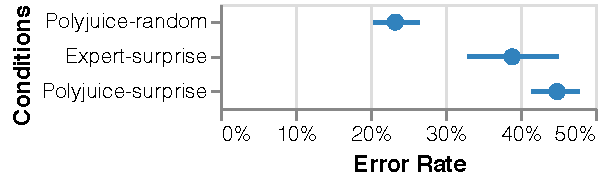
\includegraphics[width=1\columnwidth]{figures/err_rate_surprise.pdf}
\vspace{-15pt}
\caption{
Simulation error rates per condition (higher the better). 
\cshap has the highest error rate, indicating these counterfactuals would add the most information to users if displayed.
}
\vspace{-10pt}
\label{fig:err_rate}
\end{figure}
% \end{comment}

%\paragraph{Results.}
As shown in Figure~\ref{fig:err_rate}, humans simulated model behavior on \cshap counterfactuals only slightly better than random guessing ($45\%\pm6\%$), \ie these examples display model behavior that is surprising to users even after seeing explanations and creating their own counterfactuals. \chuman also had a high error rate, but at a much higher cost: generating these for just 20 original instances took 1.5--2 hours of expert labor.

While high error rates could be achieved with unrelated or nonsensical examples, all counterfactuals under evaluation were close to the original examples, when measured by syntactic tree edit (${\approx}1.0$) or Levenshtein distance (${\approx}0.2$), \cshap being the closest on both. An independent rater labeled $95\%$ of \cshap counterfactuals as ``likely written by a native speaker,'' in contrast to $85\%$ for \chuman, indicating that experts sometimes resorted to ungrammatical or nonsensical sentences to find surprising behaviors.

% Have to decide if it's worth keeping this paragraph
Qualitatively, the study participants tended to create counterfactuals by perturbing the token with the highest weights (84\% of their $\xp$ perturbed tokens in the top 15\% quantile of weights), not gaining a real understanding of how the other tokens impact predictions. Participants also made a significant number of mistakes even for tokens they had inspected, \eg a participant perturbed the example in Figure~\ref{fig:explanation}A by replacing \swap{help}{play with}, yielding a \emph{Non-Duplicate} model prediction. When faced with \swap{help}{find} in Figure~\ref{fig:explanation}D, they incorrectly assumed the behavior would be the same.

These results indicate that \sysname{} counterfactuals complement feature attribution explanations by displaying information that users often miss, even after they have manually explored the model behavior \emph{beyond} explanations. Moreover, \sysname{} counterfactuals for this application were more surprising and fluent than \chuman, despite being computed automatically.

% All the counterfactuals were close to the original examples, both in terms of the syntactic tree edit distance (0.97 in \cshap, to 1.25 in \chuman) and Levenshtein distance (around 0.2 in all conditions).
% \wts{remove Levenshtein here or add it to intrinsic evaluation part. this is what's used in MiCE.}

% As a within-subject study, we compared the error rate of human simulations across the three conditions.
% Participants only did slightly better than random guess on \cshap cases, with error rate $e=45\%\pm6\%$.
% If presented, these counterfactuals should bring more insights than hiring an expert graduate student to create counterfactuals ($e=39\%\pm11\%$), and more effectively: each graduate student had to spend 1.5--2 hours to generate 20 ``abnormal'' counterfactuals. 
% \crandom cases can be easily simulated ($e=23\%\pm6\%$), indicating the importance of abnormal counterfactuals.

% Another graduate student rated the fluency of counterfactuals, and verified that the simulation failure was not due to nonsensical noise.
% Interestingly, the rater deemed more than 95\% counterfactuals to be likely written by native speakers in both \sysname conditions, but only 85\% for \chuman, indicating that humans wrote ungrammatical sentences in order to find puzzling behavior.

% Participants' manual analysis revealed that they mostly erred when they missed the inspection spot.
% They focused mostly on what SHAP explanations deemed important, and ignored what was unimportant --- 84\% of their querying counterfactuals perturbed the most important features in the instance.\footnote{Tokens with weights higher than the 85\% quantile of all the weights in the instance.}
% For example, they repeatedly perturbed ``depression'' in Figure~\ref{fig:explanation}A, and therefore had to guess when simulating Figure~\ref{fig:explanation}B.
% In their survey responses, 7 participants explicitly stated their focus on important features, confirming that feature attributions can lead to incomplete comprehension.

% There are also 24\% of the missed \cshap cases where participants only partially inspected the related pattern,\footnote{At least one of their queries perturbed the same spans as $\xp$, and query text overlaps with the $\xp$ for over 70\%.} and were misled by it --- ``followed similar examples I tried,'' as one subject articulated.
% They could not to imagine the model predicting \emph{Duplicate} on Figure~\ref{fig:explanation}B (\swap{help}{find}), when it predicted \emph{Non-Duplicate} on their query \exinline{How do I \swap{help}{play with}...?}
% The number dropped to $15\%$ for the \chuman condition, showing that \cshap found more bugs in spots that participants considered inspected.

% \subsection{Discussions}

% \sysname counterfactuals is preferable over hiring a second expert analyst: they help find more insights at lower annotation cost, with less ungrammatical changes, and help extend manual inspection more exhaustively.
% However, certain forms of explanation selection is necessary to overcome the obvious ones. 
% The abnormality is one useful criteria that aligns with humans' cognitive processes, but humans should also be able to drive the selection, and acquire concrete foils for any spans \emph{they} do not understand.
% For example, an analyst can \texttt{BLANK} ``friend'' in Q2 in Figure~\ref{fig:explanation}C, and observe the model's unstable behavior: it predicts \emph{Non-duplicate} when \remove{friend} is changed to \add{woman}, \add{professional}, but remains \emph{Duplicate} at \add{man}, \add{student}.
% We discuss the interactions in \S\ref{sec:err_analysis}.

% As \citet{miller} noted, individual users should require less explanation the more they interact with a system.
% The fact that \sysname can still complement users' mental models, even after they see the feature attributions and manually inspect the model, indicates that the gain can be more prominent when such explanation and model access is not available. 
% We envision that the abnormality selection can also help select standalone explanations, if the expectation is instead estimated without feature attribution explanations (\eg he distance in the latent space~\cite{reimers-2019-sentence-bert}).
% We defer the exploration to future work.
